%&pdflatex
\documentclass[11pt, a4paper]{article}
\usepackage{graphicx}
\usepackage{amsmath}
\usepackage{listings}
\usepackage{minted}
\usepackage{physics}

\title{EE2703 Applied Programming Lab - Assignment No 6}
\author{
  \textbf{Name}: Abishek S\\
  \textbf{Roll Number}: EE18B001
}\date{\today}
\begin{document}
		
\maketitle 
\section{Abstract}
The goal of this assignment is the following :
\begin{itemize}
\item To characterize and analyze LTI Systems using Laplace Transform.
\item To realise low pass filters using RLC circuits.
\item To understand the use of scipy.signals toolkit.
\item To plot graphs and understand the Laplace Transform.
\end{itemize}
\usemintedstyle{manni}

\section{Assignment}
\subsection{Setting up the Program}
Importing the standard libraries
\begin{minted}[mathescape,escapeinside = ||]{python3}
import pylab as pl
import numpy as np
import sys
import scipy.signal as sp
import matplotlib
\end{minted}
We define a utility function for making plotting simpler :
\begin{minted}{python3}
def PLOT(x,y,fig_no = 0,label_x = r'$\rightarrow$',label_y = r'$\rightarrow$',
  fn = pl.plot,arg3 = 'b-',title = "Plot",grids = True,
  cmap = matplotlib.cm.jet,label = ''):
	pl.figure(fig_no)
	pl.grid(grids)
	if fn == pl.contourf:
		fn(x,y,arg3,cmap = cmap)
		pl.colorbar()
	else:
		if label == '':
			fn(x,y,arg3)
		else:
			fn(x,y,arg3,label = label)
			pl.legend()
	pl.xlabel(label_x,size = 17)
	pl.ylabel(label_y,size = 17)
	pl.title(title)
\end{minted}
We also define a utility function for making Bode Plots :
\begin{minted}{python3}
def bodeplot(w,s,phi):
    '''Makes Bode Plots'''
    plt.subplot(2,1,1)
    plt.semilogx(w,s)
    plt.xlabel(r'$\omega$',size=17)
    plt.ylabel(r'$|H(j\omega)|$',size =17)
    plt.subplot(2,1,2)
    plt.semilogx(w,phi)
    plt.xlabel(r'$\omega$',size=17)
    plt.ylabel(r'$\angle(H(j\omega))$',size =17)
\end{minted}

\subsection{Single Spring System}
\subsubsection{Varying the Decay rate of the Input - QNs 1,2}
{
We use the Laplace transform to solve a simple spring system.
The system is characterized by the given differential equation.
\[\dv[2]{x}{t} + 2.25x = f(t) \]
(Initial Conditions all are zero)\\
The Laplace transform is of the form
\[H(s) =  \frac{1}{s^2+2.25}\]
The input signal is of the form 
\(f(t) = \cos{(\omega t)}\exp(-at)u(t)\),
where a is the decay factor and $\omega$ is the frequency of the cosine.\\
The Laplace Transform of the input signal is
\[ F(s) = \frac{s+a}{(s+a)^2+\omega^2 }\]
We first use numpy polynomials to define the input, zero state response,transfer function and output in Laplace domain. 
\\The output of the system is \textbf{Zero Input + Zero State response}, where Zero Input response is Transfer function * F(s).
\\Once we get the output in Laplace domain, we take it's Inverse Laplace Transform (ILT) using \textbf{sp.impulse} to get the time domain sequences and we plot these.
We do this for $\omega$=1.5 (natural frequency of the system), and decay rate of 0.5 and 0.05.
\\We plot the outputs for $0 <= t <= 50$.
}
\begin{minted}{python3}
def input_fn(decay=0.5,cos_term=1.5):
	'''Laplace Tranform of input function'''
	return (np.poly1d([1,decay]),
		np.poly1d([1,2*decay,decay**2 + cos_term**2]))

def transfer_fn(a=1,b=0,c=2.25):
	'''Transfer function of system
	for (a*s^2 + b*s + c)*X(s)'''
	return (np.poly1d([1]),np.poly1d([a,b,c]))

def zero_st(a=1,b=0,c=2.25,xi=0,xii=0):
	'''Zero state Response of system
	for (a*s^2 + b*s + c)*X(s) with x(0) = xi and dx/dt at t = 0 is xii'''
	return (np.poly1d([a*xi,b*(xi+xii)]),np.poly1d([a,b,c]))

def output_fn(F,a=1,b=0,c=2.25,xi=0,xii=0):
	'''Laplace Transform of system output
	where F is input in Laplace domain'''
	ziN,ziD = zero_inp(a,b,c)
	zsN,zsD = zero_st(a,b,c,xi,xii)
	return (np.polyadd(np.polymul(F[0],ziN),np.polymul(F[1],zsN)),
		np.polymul(F[1],ziD))

t = np.linspace(0,50,200)

#Plotting the output (x) for decay rate = 0.5 (Qn1)
t,x1 = sp.impulse(output_fn(input_fn()),None,t)
PLOT(t,x1,1,r'$t\rightarrow$',r'$x(t)\rightarrow$',
	title = 'System response for decay rate = 0.5')
pl.show()

#Plotting the output (x) for decay rate = 0.05 (Qn2)
t,x2 = sp.impulse(output_fn(input_fn(decay=0.05)),None,t)
PLOT(t,x2,2,r'$t\rightarrow$',r'$x(t)\rightarrow$',
	title = 'System response for decay rate = 0.05')
pl.show()

\end{minted}
\begin{figure}[H]
   	\centering
   	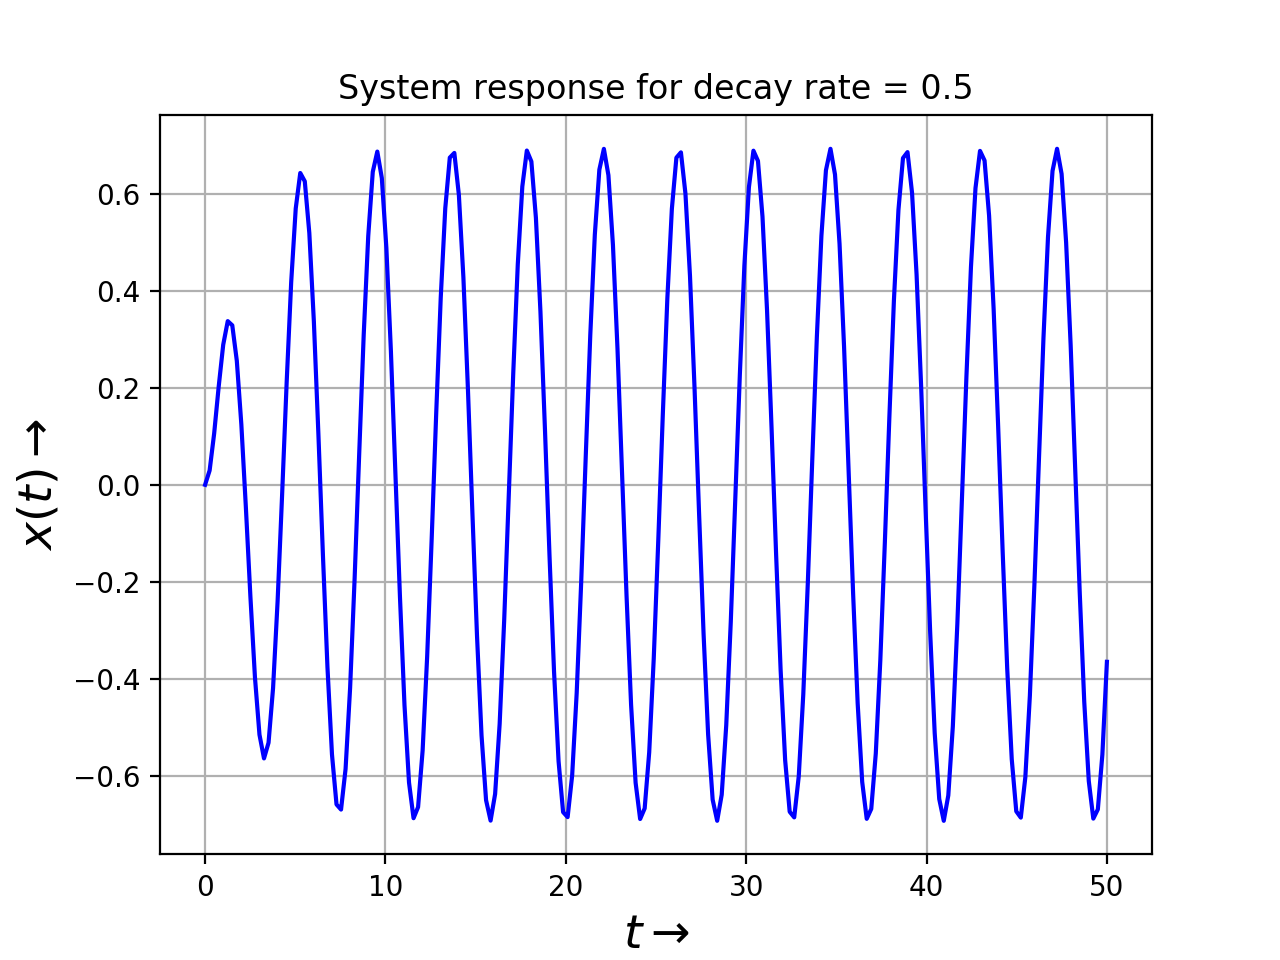
\includegraphics[scale=0.6]{ss5.png}
   	\label{fig:ss0.5}
   	\caption{System Output for decay rate = 0.5}
\end{figure}
\begin{figure}[H]
   	\centering
   	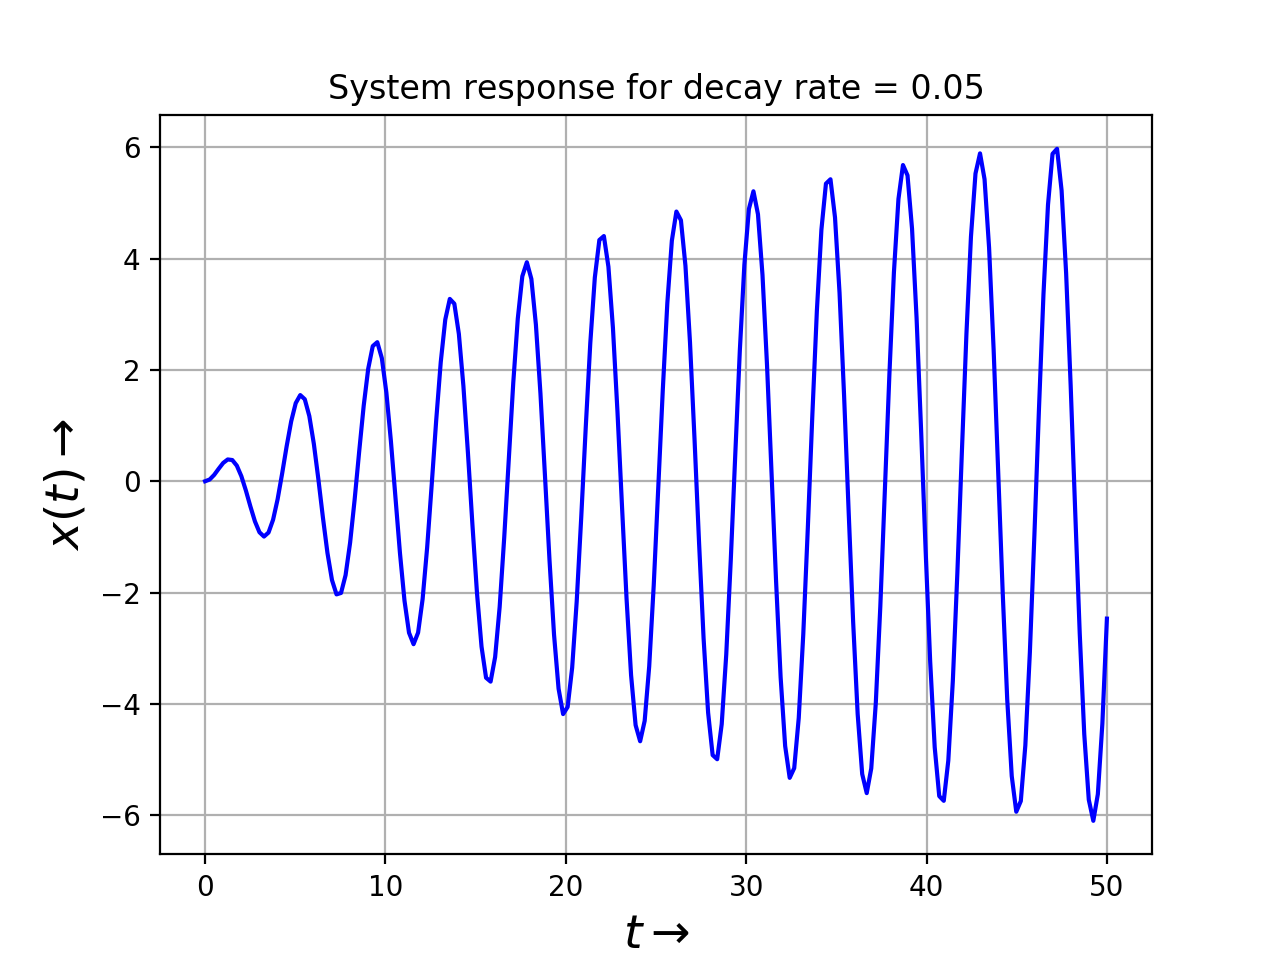
\includegraphics[scale=0.6]{ss05.png}
   	\label{fig:ss0.05}
   	\caption{System Output for decay rate = 0.05}
\end{figure}
{
We observe that the \textbf{oscillation amplitude settles to a fixed value} in both the cases.
\\We observe it \textbf{takes longer to settle when the decay rate is less}.
\\We also note that the \textbf{amplitude increases to a much larger amount in the case with lower decay rate}.
\\At zero decay rate the amplitude increases to infinity, and at high decay rate the output reaches the maximum amplitude almost instantaneously.
}

\subsubsection{Varying the frequency of the input - QN 3}
We first define a \textbf{input\_td} function which gives the input values in time domain corresponding to the time values passed to it.
\begin{minted}{python3}
def input_td(t,decay=0.5,cos_term=1.5):
	'''Return list of input values in time domain 
		corresponding to the t values given'''
	return (np.cos(f*t)*np.exp(-1*decay*t))
\end{minted}
{
We vary the frequency of the cosine term in input and analyse it's effect.
\\We plot the outputs for $0 <= t <= 100$.
\\We also construct the bode plot of the transfer function to understand the results in a better way.
}
\begin{minted}{python3}
t = np.linspace(0,100,300)
H = transfer_fn()

#We use the following 5 colours for the lines :
#Black Green Red Cyan and Magenta
for f,col in zip(np.arange(1.4,1.61,0.05),['k','g','r','c','m']):
	u = input_td(t,0.05,f)
	t,y,svec = sp.lsim(H,u,t)
	PLOT(t,y,3,r'$t$',r'$x(t)$',
		title = 'System responses for different frequencies 
		with decay rate = 0.05',arg3 = col+'-',label = 'freq '+str(f))

pl.show()

#We make the Bode plot of the transfer function to understand it better
w,s,phi = sp.lti(H[0],H[1]).bode()
pl.figure(4)
pl.title('Bode plot of Transfer function of single spring system')
bodeplot(w,s,phi) 
pl.show()

\end{minted}
\begin{figure}[H]
   	\centering
   	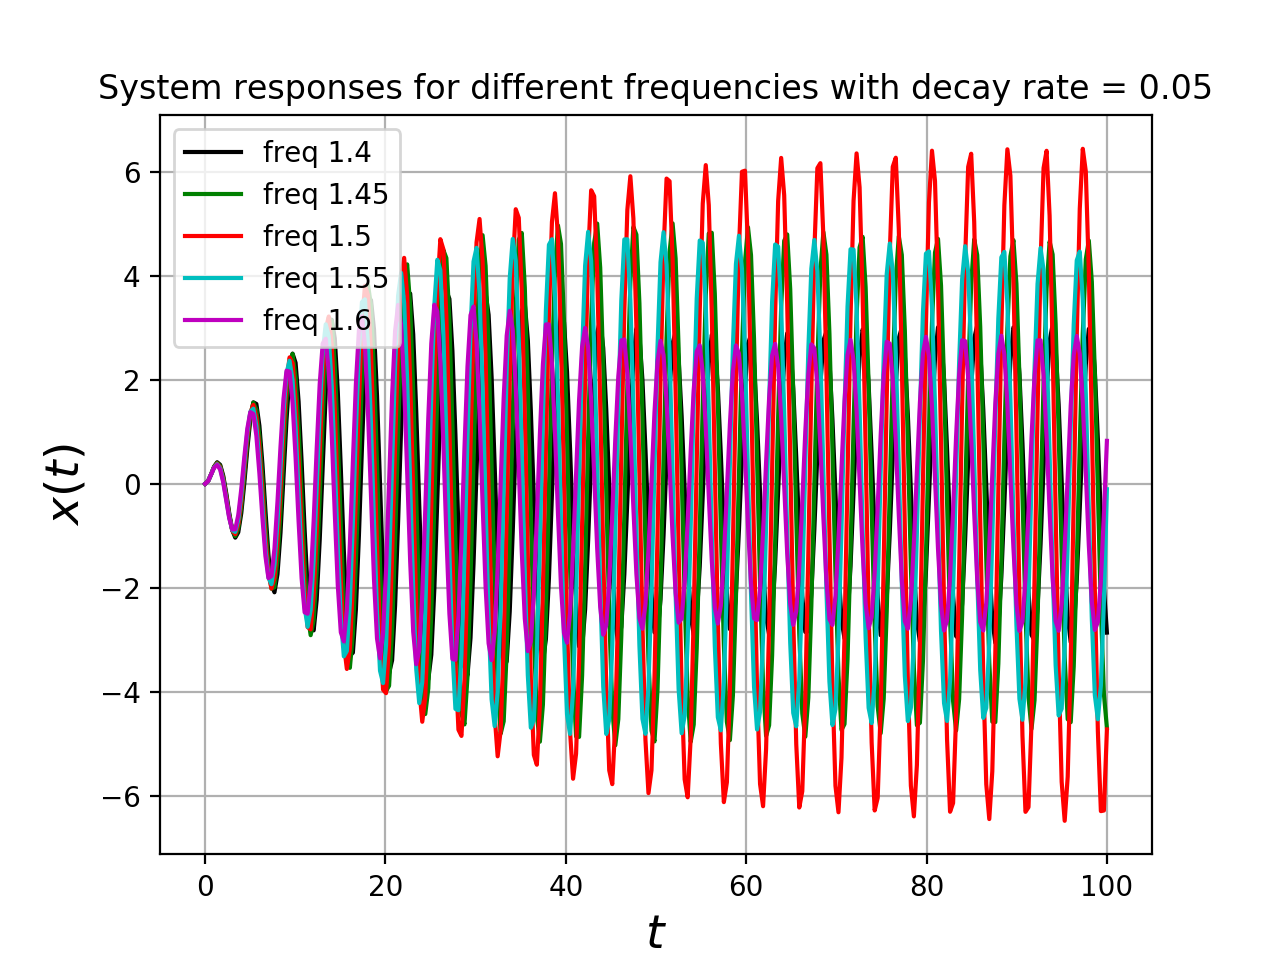
\includegraphics[scale=0.6]{ss_freq.png}
   	\label{fig:ss_freq}
   	\caption{System Output for different frequencies at decay rate = 0.05}
\end{figure}
\begin{figure}[H]
   	\centering
   	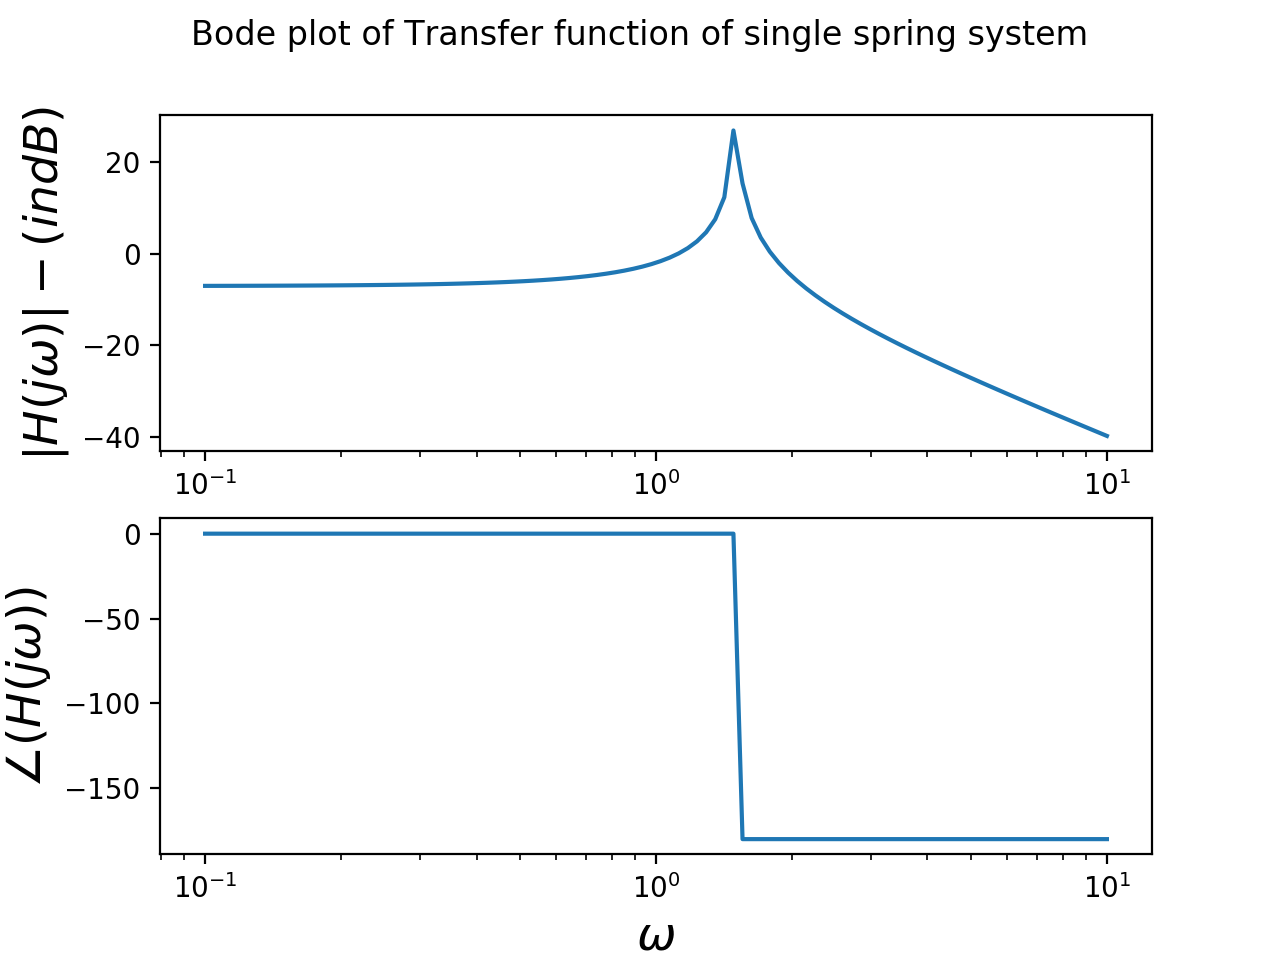
\includegraphics[scale=0.8]{bode_ss.png}
   	\label{fig:bode_ss}
   	\caption{Bode Plot of Transfer function (both magnitude and phase)}
\end{figure}
{
When the \textbf{input frequency is equal to the natural frequency the output amplitude is maximum}.
\\In the other cases the output amplitude is less than that.
This phenomenon can be attributed to \textbf{Resonance}.
\\
We can also clearly see from the bode plot that there is a maximum at the natural frequency, and there is a second order pole there, as the phase shift is $-180\deg$.
}

\subsection{Coupled Spring System - QN 4}
{
We have two differential equations and two variables to solve for.
The equations are :
\[\dv[2]{x}{t} +(x-y) = 0 \]
\[\dv[2]{y}{t} +2(y-x) = 0 \]
with  initial conditions for x (some are given, others can be obtained by substituting in the given equations) :
\[x(0) = 1\]
\[x^{(1)}(0) = 0\]
\[x^{(2)}(0) = -1\]
\[x^{(3)}(0) = 0\]
We substitute y in the second equation from the first, and we get a fourth order differential equation in terms of x.
Simplifying this and substituting to find y, we get :
\[X(s) = \frac{s^2+2}{s^3+3s} \]
\[Y(s) =  \frac{2}{s^3+3s} \]
We can take the ILT of these two expressions to find the time domain expressions for x(t) and y(t).
We plot these for $0 <= t<= 20$ in one graph.
}
\begin{minted}{python3}
t = np.linspace(0,20,200)
#Transfer function for x
X = sp.lti([1,0,2],[1,0,3,0])

#Transfer function for y
Y = sp.lti([2],[1,0,3,0])

t,x = sp.impulse(X,None,t)
t,y = sp.impulse(Y,None,t)

#Plotting x(t) and y(t) in a single graph
PLOT(t,x,5,'t','f(t)',title = 'Plot of x(t) and y(t) in coupled spring system',
	label = 'x(t)')
PLOT(t,y,5,'t','f(t)',title = 'Plot of x(t) and y(t) in coupled spring system',
	arg3 = 'g-',label = 'y(t)')
pl.show()

\end{minted}
\begin{figure}[H]
   	\centering
   	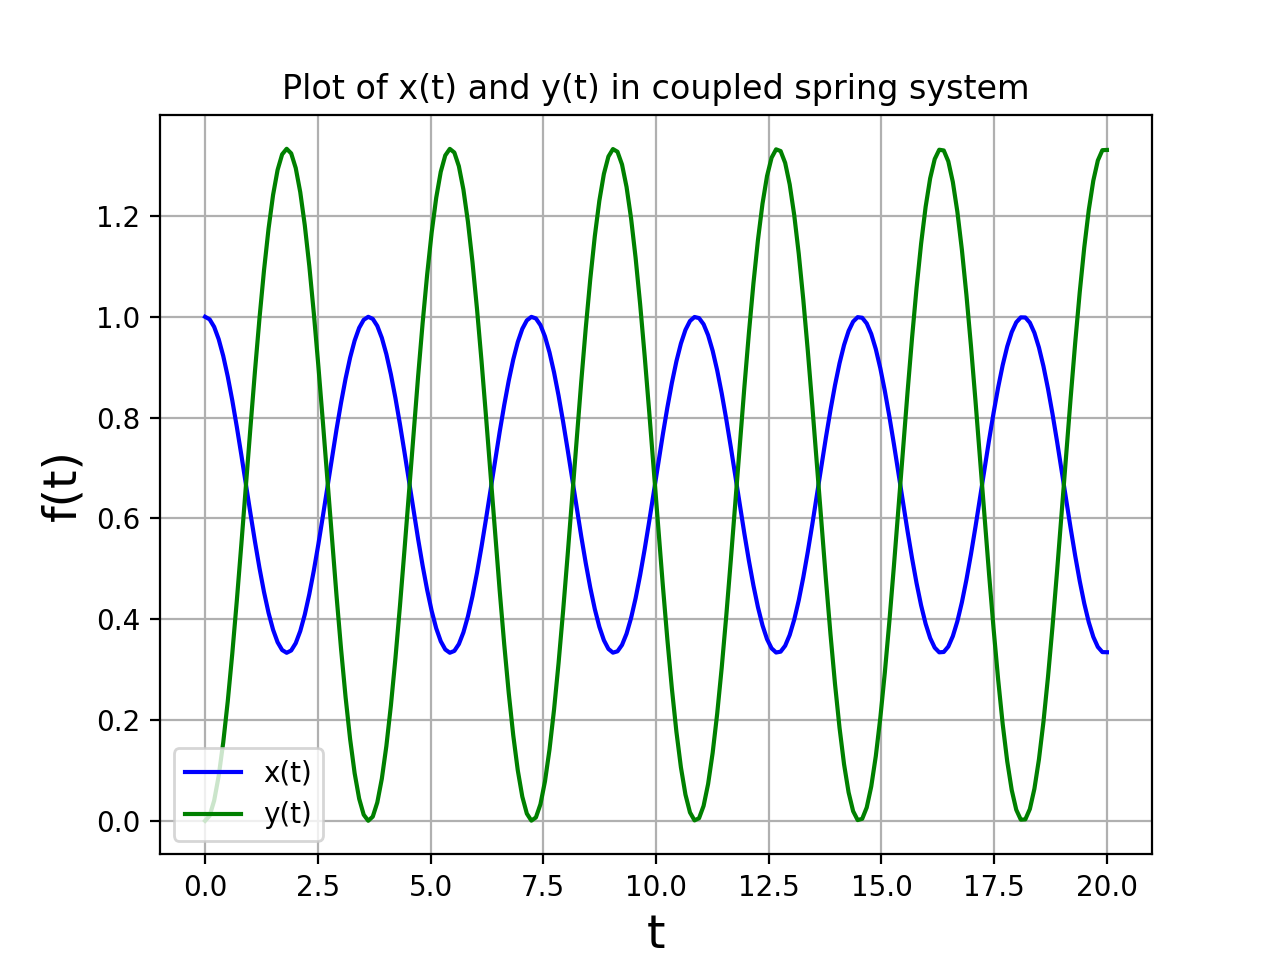
\includegraphics[scale=0.6]{cs_xy.png}
   	\label{fig:cs_xy}
   	\caption{x(t) and y(t) in coupled spring system}
\end{figure}
{ 
We observe that the \textbf{amplitude of y is greater than x}. 
\\They are \textbf{opposite in phase}.
\\They oscillate about the same mean point.
\\This models two masses attached to the ends of an ideal spring.
}

\subsection{RLC Filter - QNs 5,6}
{
We now consider an RLC Filter with transfer function calculated as :
\[ H(s) = \frac{1}{10^{-12}s^2 + 10^{-4}s + 1}\]
(Initial Conditions all zero)
\\We define a function to return the Transfer function of the RLC circuit in \textbf{np.poly1d} form :
\begin{minted}{python3}
def RLCtf():
	'''Transfer function of the RLC circuit given'''
	return (np.poly1d([1]),np.poly1d([1e-12,1e-4,1]))
\end{minted}
We then make the Bode plot of the Transfer function.
\begin{minted}{python3}
#Defining time vector appropriately from 0 to 10msec with 1e-7 time steps 
	to cpature the fast variation
t = np.arange(0,10e-3,1e-7)
H = RLCtf()

w,s,phi = sp.lti(H[0],H[1]).bode()
pl.figure(4)
bodeplot(w,s,phi) 
pl.suptitle('Bode plot of Transfer function of RLC filter')
pl.show()

\end{minted}
{
From the Bode plot, it is clear that the RLC System is a \textbf{second order Low Pass Filter}.
}
\\
The input is of the form
\[x(t) = \cos{(10^3t)}+\cos{(10^6t)} \]
which is the superposition of two sinusoids with low and high frequencies of $10^3$ and $10^6$ respectively.
\\We define another function that returns the input to the RLC circuit :
\begin{minted}{python3}
def RLCinp():
	'''Input to the RLC circuit'''
	return (np.cos(1e3*t)-np.cos(1e6*t))
\end{minted}
We use \textbf{sp.lsim} to find the output of the filter, which will be convolution between input and ILT of the Transfer function.
We plot the output from 0 to 30$\mu$s (to capture the \textbf{Fast time} part) as well as from 0 to 10ms (to capture the \textbf{Slow time} part).
}
\begin{minted}{python3}
#Solving for the RLC filter output
u = RLCinp()
t,x,svec = sp.lsim(H,u,t)

#Plotting the slow time and fast time outputs separately
PLOT(t,x,6,'t','V(t)',title = 'Plot of Output voltage of
	RLC circuit - Slow time')
pl.show()
PLOT(t[:300],x[:300],7,'t','V(t)',title = 'Plot of Output voltage of 
	RLC circuit - Fast time')
pl.show()

\end{minted}
\begin{figure}[H]
   	\centering
   	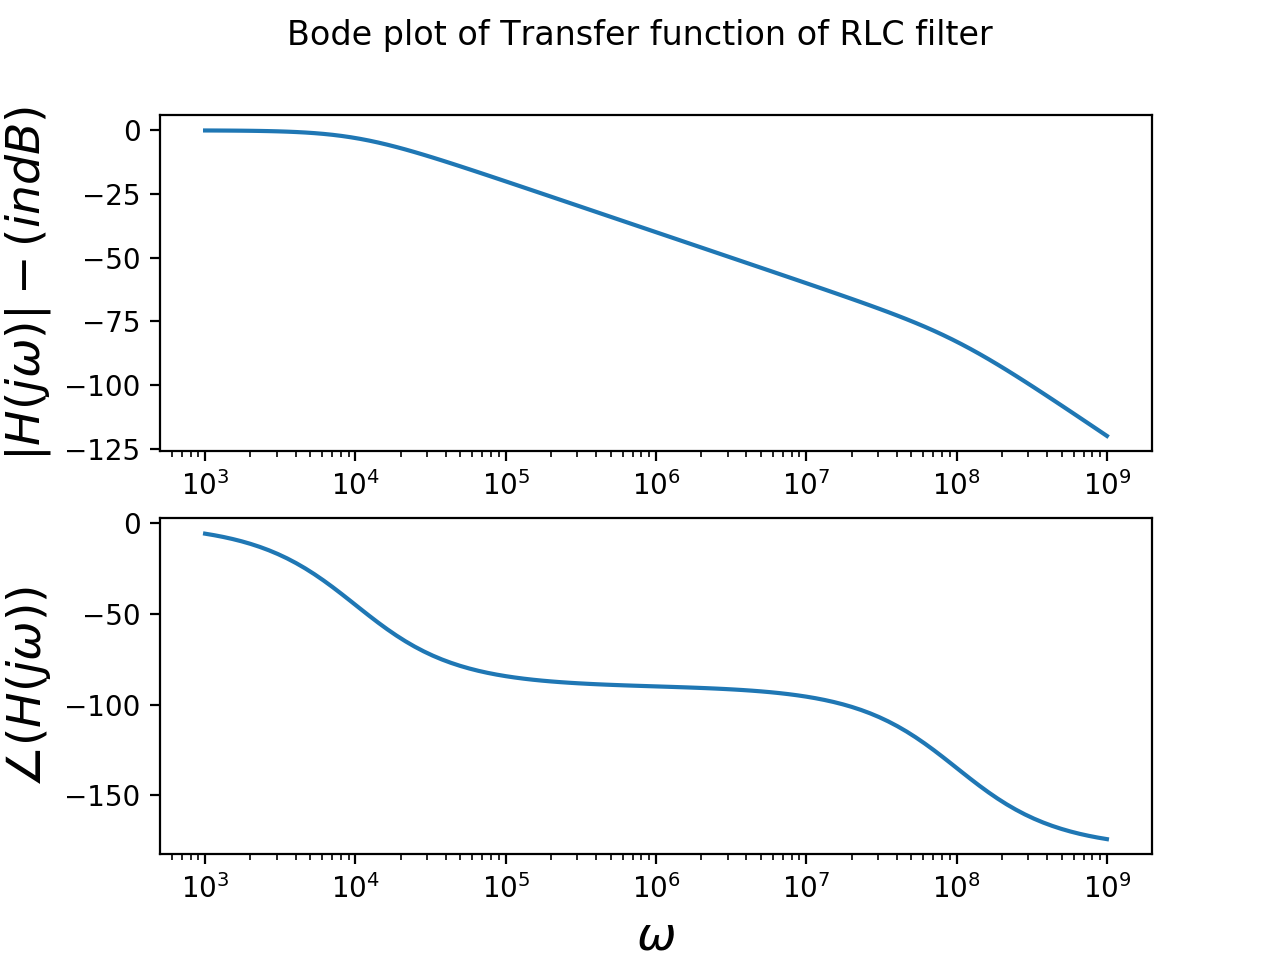
\includegraphics[scale=0.8]{bode_rlc.png}
   	\label{fig:bode_rlc}
\end{figure}
\begin{figure}[H]
   	\centering
   	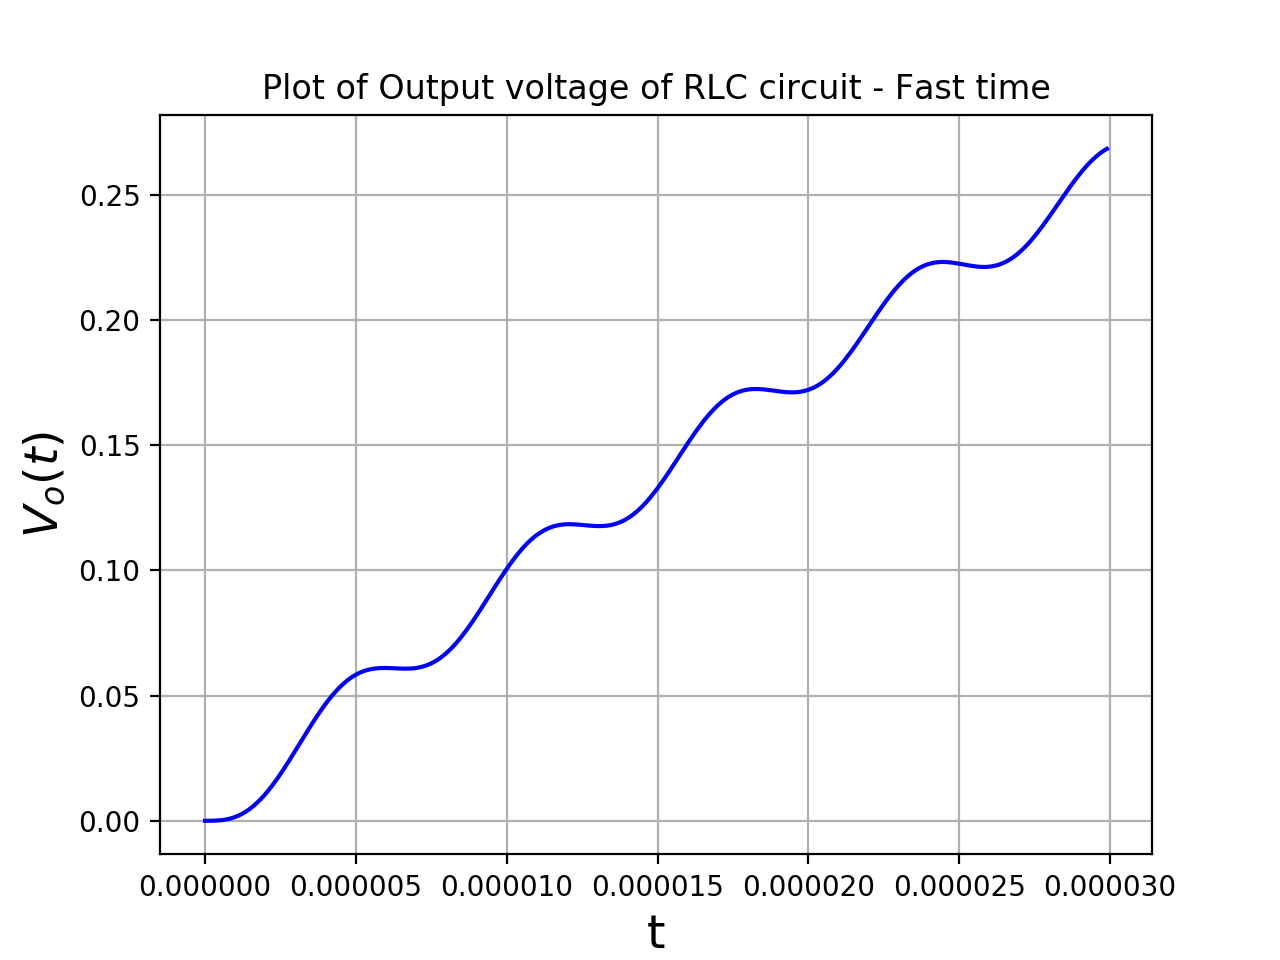
\includegraphics[scale=0.6]{RLC_fast.png}
   	\label{fig:RLC_fast}
   	\caption{RLC Circuit - Plot of Output Voltage - Fast Time}
\end{figure}
\begin{figure}[H]
   	\centering
   	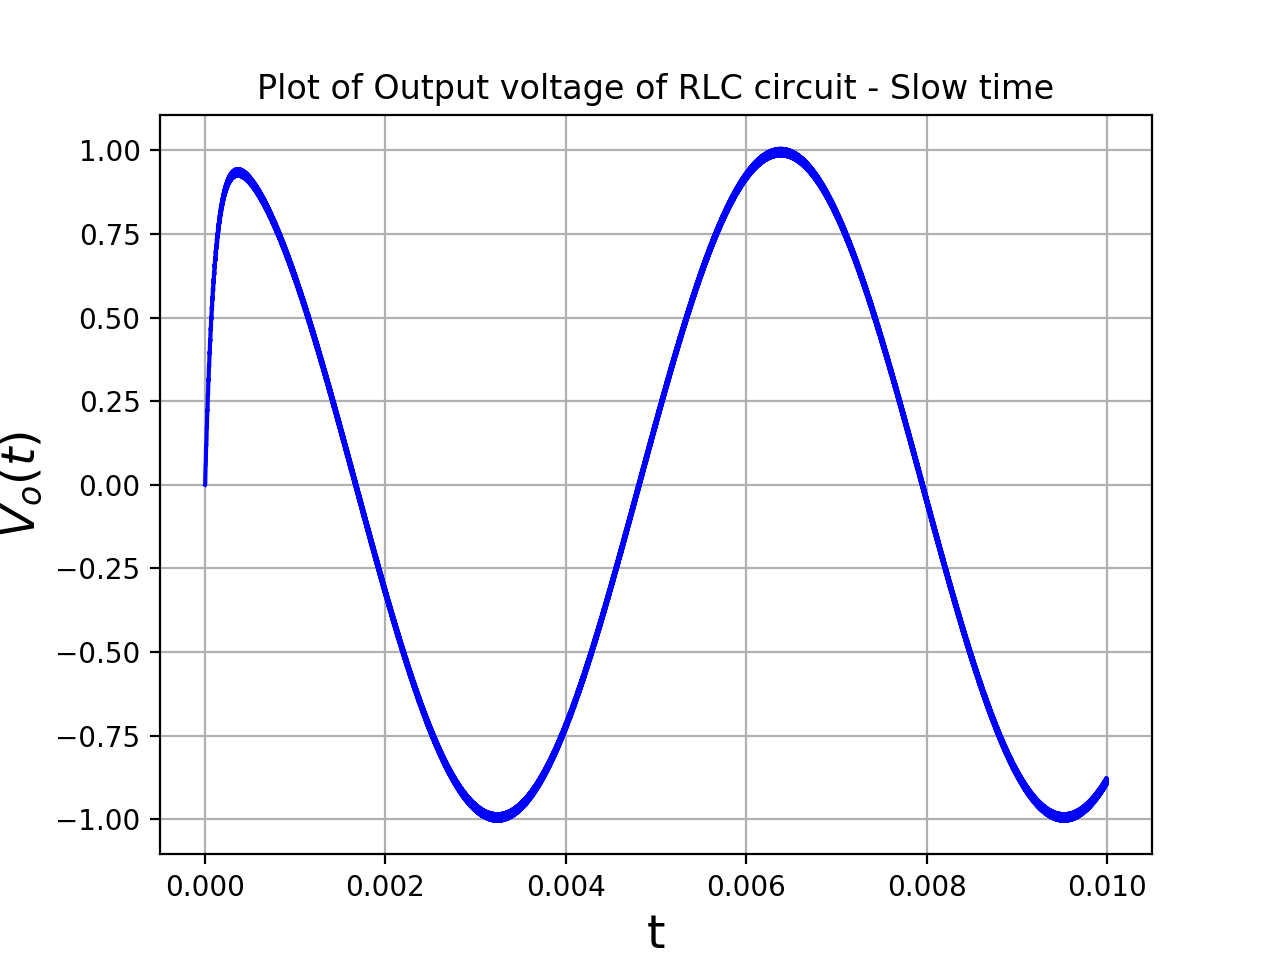
\includegraphics[scale=0.6]{RLC_slow.png}
   	\label{fig:RLC_slow}
   	\caption{RLC Circuit - Plot of Output Voltage - Slow Time}
\end{figure}
{
The fast time plot shows that the \textbf{capacitor is charging up} to meet the input amplitude. 
\\The high frequency component can be seen as a \textbf{ripple} in the fast time plot.  This component is highly attenuated and hence not visible in the slow time plot.
\\In the slow time plot, we notice that the low frequency component passes almost unchanged, the amplitude is nearly 1.
The reason for this is that $\omega = 10^3\frac{rad}{s}$ is well within the 3-dB bandwidth ($\omega_{3dB} \approx 10^4\frac{rad}{s}$) of the system.
This reiterates the fact that this is a low pass filter with bandwidth $\omega_{3dB} \approx 10^4\frac{rad}{s}$.
}

\section{Conclusions}
\begin{itemize}
\item We  modelled the spring system and RLC circuit as LTI systems and analysed them using Laplace Transforms.
\item We observed how a RLC circuit can behave as a Low Pass Filter.
\item We used the scipy signals toolkit to construct Bode Plots and calculate time domain response and convolutions.
\item We plotted graphs and Bode plots to understand the behaviour of those LTI systems.
\end{itemize}

\end{document}